\documentclass{iitthesis}

%   \documentclass[draft]{iitthesis}

%\usepackage[dvips]{graphicx}    % This package is used for Figures
\usepackage{graphicx}    % This package is used for Figures
\usepackage{rotating}           % This package is used for landscape mode.
\usepackage{epsfig}
\usepackage{subfigure}          % These two packages, epsfig and subfigure, are used for creating subplots.
\usepackage{mathtools}          
% Packages are explained in the Help document.


\begin{document}
%%fakesection{TITLES AND INDEXES)
%%% Declarations for Title Page %%%
\title{Energy saving for UAV flight in gusting conditions \\
through trajectory optimization \\
and active flow control}
\author{Lou Grimaud}
\degree{Master of Science}
\dept{Mechanical, Materials, and Aerospace Engineering}
\date{May 2014}
%\copyrightnoticetrue      % crate copyright page or not
\maketitle                % create title and copyright pages


\prelimpages         % Settings of preliminary pages are done with \prelimpages command


%%%  Acknowledgement %%%
\begin{acknowledgement}     % acknowledgement environment, this is optional
\par  This dissertation could not have been written without Dr. X
who not only served as my supervisor but also encouraged and
challenged me throughout my academic program. He and the other
faculty members, Dr. Y and Dr. Z, guided me through the
dissertation process, never accepting less than my best efforts. I
thank them all.\\ \\ (Don't copy this sample text. Write your own
acknowledgement.)
%\input{acknowledgement.tex} % you need a separate acknowledgement.tex file to include it.
\end{acknowledgement}


% Table of Contents
\tableofcontents
\clearpage

% List of Tables
\listoftables

\clearpage

%List of Figures
\listoffigures

\clearpage

%List of Symbols(optional)

\listofsymbols
 \SymbolDefinition{$\beta$}{probability of non-detecting bad data}
 \SymbolDefinition{$\delta$}{Transition Coefficient Constant for the Design of Linear-Phase FIR Filters}
 \SymbolDefinition{$\zeta$}{Reflection Coefficient Parameter}


 \clearpage

%%% END OF INDEXES %%%
%%%%%%%%%%%%%%%%%%%%%%%%%%%%%%%%%%%%%%%%%%%%%%%%%%%%%%%%%%%%%%%%%%%%%%%%%%%%%%%%%%%%%%%

%%% Abstract %%%
\begin{abstract}           % abstract environment, this is optional
 \par The purpose of this thesis is to show how micro unmanned aerial vehicles can extract energy from natural wind gusts and how this energy extraction is affected by the effects of unsteady aerodynamics.

\par The trajectory of a small UAV flying through wind gusts is simulated with a two degrees of freedom model.
The non-dimensional model is set to include vertical and horizontal gusts of varying amplitudes and durations.
From this model an optimization routine is performed in order to obtain the minimum gust amplitude needed to get a neutral energy trajectory.
With these results, it is shown that neutral energy flight is possible through gusts speeds only 10 to 30\% of the flying speed of the aircraft .
Analysis of the results shows that the lift coefficient has to be changed very rapidly in order to perform these maneuvers in short duration gusts. 
Moreover high lift values are often required. 

\par To achieve this kind of rapid changes in the lift and drag forces, fast variations of the angle of attack are needed.
The high lift values also requires high angles of attacks that are likely to cause separation of the flow over the airfoil.
These fast variations at high angle of attack are shown to cause unsteady non linear aerodynamic responses.
Traditional CFD simulations are far too computationally expensive to be implemented into the optimization routine.
To solve this issue a low order model based on a paper by Goman and Khrabrov \cite{GK} is developed and validated against experimental results.
This model produces accurate predictions of the lift and drag coefficients for a wide range of angle of attack and for different type of pitch inputs.

\par With this light model the influence of the unsteady aerodynamics on the energy extraction problem are highlighted.
The main difference with quasi-steady aerodynamics model was found to be for gusts at a reduced frequency faster than k of 0.07.
Around these values the potential performances are improved by introducing the unsteady model.
The trajectories obtained include more violent changes in angle of attacks in order to take full advantages of the unsteady effects.



  %you need a separate abstract.tex file to include it.
\end{abstract}


\textpages     % Settings of text-pages are done with \textpages command

% Chapters are created with \Chapter{title} command
\Chapter{INTRODUCTION}

\Section{Motivations} \label{subsec:dynsoar}

\Subsection{Trajectory optimization through wind gusts}
The main challenge for electric small size unmanned aerial vehicle is the autonomy.
Battery energy density is limited and can rapidly become a important part of the weight of vehicle.
Since most of the energy is used by the electric engine for propulsion, optimizing the control laws and trajectory could have a dramatic effect on endurance. 
With the progress in autonomous control software successful attempt have been made by Allen \cite{flight_test_soaring_NASA} and Edwards \cite{flight_test_soaring_NCU} to extract energy from natural updraft.
These experiments have shown that an UAV can take advantage of localized vertical winds naturally produced by thermal convection.

\par However, within an urban environment, such as the one mini and micro-UAV are made for, the gust's profile is vastly different. 
Wind blowing through an group of building produce turbulent conditions with both vertical and horizontal vortexes.
These turbulences can reach speed representing a significant portion of micro-UAV's glide speed. 
In flow fields such as this the gusts encountered are both faster and arguably more complex than the ones due to thermal convection.

\par The lack of low order models for the unsteady effects meant that all of the studies on trajectory optimization seemed to have focused on quasi-steady models to compute the aerodynamic forces.
More computationally expensive model traditionally used for CFD are too unpractical considering the thousands of functions evaluations needed for such algorithm.
To solve this problem a low order model capturing the unsteady behavior of the flow over the aircraft is needed.
Additionally this model needs to be able to handle flow separation and airfoil stalling since the maneuvers required for energy extraction can be relatively violent and often involve high angle of attack.


\Subsection{Pitching airfoil model}
The difficulty is that the lift and drag behavior in such condition is time dependent and non-linear.
As such finite elements methods are often the only solution to get a good simulation of the lift and drag.
Such solution are useful since they provide a lot of information about the flow flied itself, but the computation time required to get the lift and drag out of them is several order of magnitude too long.

\par Another solution explored by Brunton \cite{brunton2008unsteady} is to perform linear approximations of the lift and drag behavior at different angles of attack.
These linear models can then be patched together to include the non-linear behaviors.
The appeal of this method is that the individual linear models can be easily analyzed using classical LTI system theory.
It is however still fairly complicated and requires an extensive experimental study to identify the system at each set angle of attack.

\par The model developed by Goman and Khrabrov allows for a low order model non linear model to capture the features of the lift coefficient over a very wide range of angle of attack as well as for any arbitrary pitch profile.
One quasi-steady map of the lift and two time constants are all that is needed to get the full model.
So far it seems that the use of this model has been limited to the lift coefficient predictions however for the trajectory optimization the drag coefficient is also needed.

\Section{Previous investigations/literature review}

\par As explained in the previous part \ref{subsec:dynsoar}, the bulk part of the research on trajectory optimization for small flying vehicle has been focused on either natural convection such as the one glider pilots and some birds of prey take advantage of in plains, or wind gradients such the ones found close to the surface of the ocean.
The later are often exploited by seabird such as albatrosses.

\par Lissaman \cite{lissaman2005wind} has conducted a study for 3D trajectories in differently shaped wind gradients close to the ground.
His optimization is performed on a non-dimensional set of equation that has been reused in this study.
He also uses different kind of profiles for the wind gradient in order to represent more accurately real wind gradients.


\Chapter{Energy extraction optimization} \label{ch:Eni_extraction}

\Section{2 DoF model}

\Subsection{Non-dimensional equations of motion}
The model chosen for this simulation is a simple two degree of freedom, two dimension, point mass model. 
The aircraft is assumed to be a glider to simplify the optimization routine. 
With such assumption the equations of motion in the ground reference frame is :

\begin{equation}
\begin{array}[c]{c}
  \ddot{x}= -L' \cdot sin(\gamma) + D' \cdot cos(\gamma) \\ 
  \ddot{z}= L' \cdot cos(\gamma) - D' \cdot sin(\gamma) - m \cdot g
\end{array}
\label{eqn:eqm}
\end{equation}

% should I include a figure with the reference frame, and angle definition?

\par The lift and drag are defined are: 

\begin{equation}
\begin{array}[c]{c}
  L'= \frac{1}{2} \rho v^2 C_l \\ 
  D'= \frac{1}{2} \rho v^2 C_d 
\end{array}
\label{eqn:Cl_def}
\end{equation}

\par With $v$ being the relative wind for the vehicle.
% do I need to include this kind basic stuff?

\par Since this simulation is mainly concerned with Newtonian physics (rather than fluid phenomenons) the usual fluid dynamics non-dimensional variables make little sense.
Here the equations are normalized by the optimal glide speed and $g$, the gravitational acceleration.
This is more representative of the performances of the aircraft.

\par Following Lissaman's \cite{lissaman2005wind} implementation of the equation of motion we define $V^*$ the optimal glide speed for the aircraft. 
This speed is achieved at the optimal lift to drag ratio of the aircraft.
With $C_l^*$ and $C_d^*$ the angle of attack for the maximum lift to drag ratio and $\gamma$ the pitch angle with respect to the horizon the optimal glide speed is:

\begin{equation}
\begin{array}[c]{c}
  \gamma^*= - atan(\frac{C_l^*}{C_d^*}) \\
  V^* = \sqrt{\frac{2mg}{\rho S (C_l^* cos(\gamma^*) - C_d^* sin(\gamma^*)}}
\end{array}
\label{eqn:glide_speed}
\end{equation}

\par From we define $U$ and $W$ the non dimensional horizontal and vertical speed in the inertial reference frame.

\begin{equation}
\begin{array}[c]{c}
  U = \frac{\dot{x}}{V^*} \\
  V= \frac{\dot{z}}{V^*}
\end{array}
\label{eqn:non_dim_speed}
\end{equation}

The time is normalized by $g / V^*$.

\par Since the speed is seen as a fraction of the optimal glide speed it makes sens to also normalize the lift and drag coefficients by their corresponding values at the optimal lift to drag ratio.

\begin{equation}
\begin{array}[c]{c}
  L= \frac{C_l}{C_l^*} \\
  D= \frac{C_d}{C_d^*} 
\end{array}
\label{eqn:non_dim_coef}
\end{equation}

\par Finally we introduce Q the dynamic pressure as:

\begin{equation}
Q = \frac{L'}{MgL} = \frac{\frac{1}{2} \rho V^2 C_l C_l^* }{Mg}
\label{eqn:dynamic_pressure}
\end{equation}

\par From there the equation of motion \ref{eqn:eqm} can be expressed as:

\begin{equation}
\begin{array}[c]{c}
  \frac{dU}{dT}= -LQ \cdot sin(\gamma) + DQ \cdot cos(\gamma) \\ 
  \frac{dW}{dT}= LQ \cdot cos(\gamma) - DQ \cdot sin(\gamma) - 1
\end{array}
\label{eqn:non_dim_eqm}
\end{equation}

With 

\begin{equation}
\gamma = -atan(\frac{W-W_g}{U-U_g})
\label{eqn:gamma_def}
\end{equation}

$W_g$ and $U_g$ are the vertical and horizontal wind speeds in the inertial reference frame.

\par Finally the remaining thing to consider is $Q$ the dynamic pressure. If we define the speed of the wind gust as $W_g$ and $U_g$ we can express:

\begin{equation}
Q = V^2 = (W-W_g)^2 + (U-U_g)^2
\label{eqn:q_def}
\end{equation}

\par With these definitions we have the basic formulation of our non-dimensional equation of motions, normalized by the performances at the optimal glide trajectory in a calm environment.

\Subsection{Lift and drag models}
The normalized equation of motion \ref{eqn:non_dim_eqm} are not accounting for the fluid dynamic part of the flight.
The most important factor for glide performance is the lift to drag ratio. 
In his paper, Lissaman \cite{Lissaman2007neutral} is using a relatively simple quadratic model for the relationship between lift and drag:

\begin{equation}
D=\frac{Q}{2G}(1+L^2)
\label{eqn:Lissaman_G}
\end{equation}

%[CHECK THIS EQUATION !!!!!]

\par This simple model work relatively well for simple airfoil but is inadequate for more complex shapes.
Moreover it fails to properly account for the effects of flow separation at high angle of attacks.
Finally this model is only valid for the quasi-steady flow conditions.

\par Since the unsteady model developed in chapter \ref{Ch:gkmodel} is based on experimental results for a NACA0009 airfoil, we will use simplified versions of the lift and drag characteristics of this airfoil.

\begin{figure}[ht]
\begin{center}
  \scalebox{0.8}
  {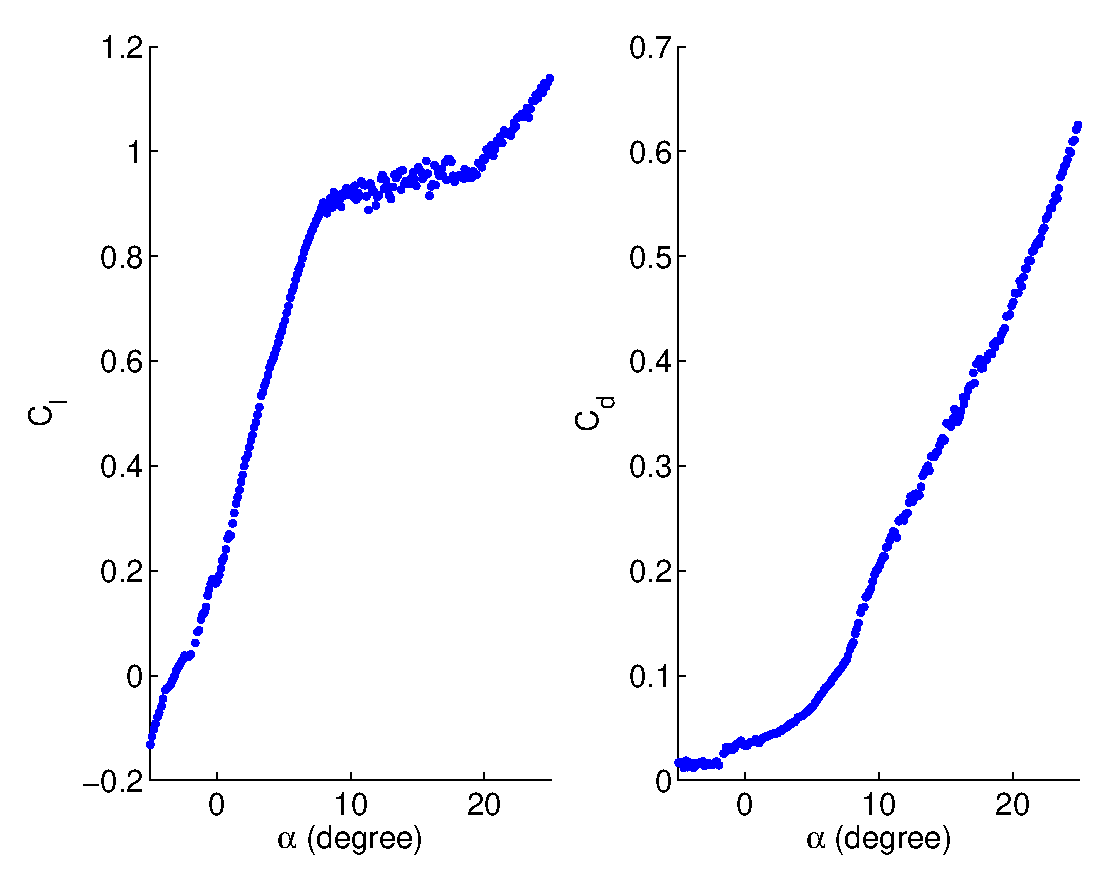
\includegraphics{./Figures/NACA0009_steady_map_Cl_Cd.eps}} 
\end{center}
\caption{Lift and drag characteristics of the NACA0009}
\end{figure}


\begin{figure}[ht]
\begin{center}
%    \scalebox{0.8}
%   {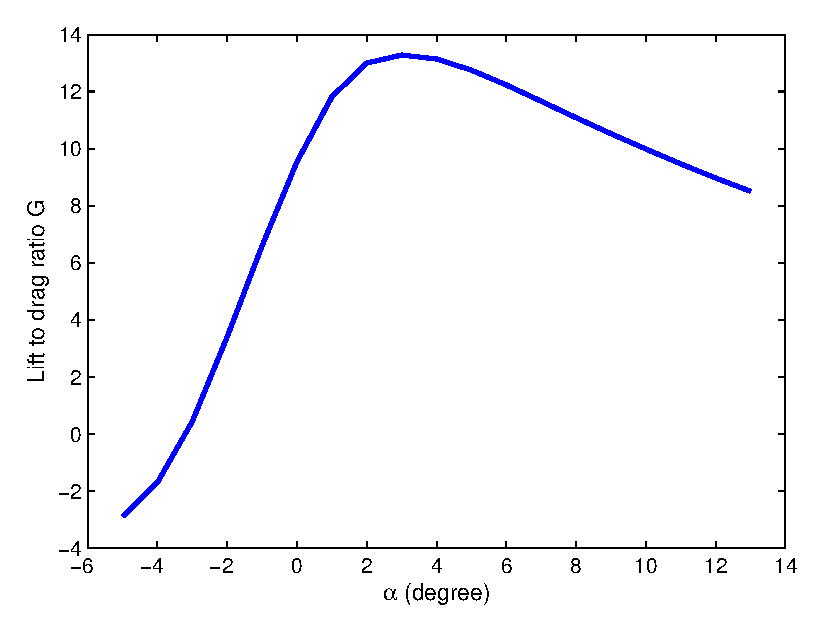
\includegraphics{./Figures/lift_to_drag_UAV.eps}}
\end{center}
\caption{Lift to drag ratio for the NACA0009}
\end{figure}

\par This results, while being arguably more realistic than a simple quadratic approach, are still only considering quasi-steady change in the angle of attack.
This limitation will be discussed more in depth in the result discussion section \ref{sec:results_QS}.

\Subsection{Wind profiles}
Most of the studies done on dynamic soaring has either been done with vertical wind gusts or thermal updraft, or horizontal wind gradient foxed in time.
In this optimization procedure we chose to consider three different wind profiles made out of first order sinusoidal gusts.

\par Our first gust profile is a simple vertical gust.

\begin{equation}
\begin{array}[c]{c}
  W_g = W_a \cdot sin(2\pi T) \\
  U_g = 0 
\end{array}
\label{eqn:vertical_gust_definition}
\end{equation}

\par Similarly the horizontal gust is defined as:

\begin{equation}
\begin{array}[c]{c}
  W_g = 0 \\
  U_g = W_a \cdot cos(2 \pi T)
\end{array}
\label{eqn:horizontal_gust_definition}
\end{equation}

\par Finally a more complex combined gust is defined.
This gust profile is the sum of the two previously defined gusts.
Moreover we introduce $\phi$, a phase difference between the two component of the gust. 

\begin{equation}
\begin{array}[c]{c}
  W_g = W_a \cdot sin(2\pi T) \\
  U_g = W_a \cdot cos(2 \pi T + \phi)
\end{array}
\label{eqn:combined_gust_definition}
\end{equation}

\Section{Optimization process, cost function and constraints}

\Subsection{General consideration on optimization}
% Get some stuff from the MM544 class
The general principle for the optimization routines resides in defining a so called ``cost function'' that will represent a quantity we want to minimize.
While the algorithm tries to minimize this scalar, a set of constraints have to be respected. 
These constraints can represent physical limitations or specific requirements related to the system at hand.
The cost and constraints are expressed as functions of a set of system state variables.
The state variables can represent temporal or spatial values.
The optimization is performed in a sequential fashion where different algorithm are used to step from one set of values for the state variables to another. 

\par Optimization routines are divided into two families. 

\par The first method is called the gradient method, it requires a good knowledge of the physics behind the problem.
The cost function as well as the constraints have to be explicitly defined.
In this method the gradient of the cost function and the constraints is used to determine the direction of the next step in the optimization.
Different algorithm are used to chose the step size, and sometime the direction of the previous step can influence the current step.
The gradients for either the cost function or the constraints do not have to be explicitly defined as modern optimization routines, such as the one included in Matlab, can perform numerical gradient estimation.
However inputting an user defined gradient into the routine will significantly speed up the overall process.

\par The second method is using the so called ``evolutionary algorithms''. 
This method relies a lot less on knowing the underlying physical phenomenon.
Its basic principle is a ``try and see'' process.
Random changes are performed on the state variables and their effects on the cost function are assessed.
The best steps are selected as a starting point for the next generation.
While with this method each step is a less computation intensive than with the previous method, the number of steps is a lot higher.

\par The first method has been used in this optimization as it provides more insight on the physics behind the problem.
However it should be noted that the resulting ``optimal'' point is usually only assured to be \emph{a local} minimum of the cost function.
Several different starting states should be tested to ensure that the optimization converges toward a reasonable minimum.



\Subsection{Cost function}
Our problem here consists in optimizing the trajectory in a gusting environment to minimize energy lose.
The most obvious cost function would be something like

\begin{equation}
  - \frac{1}{2}m{V(T_f)}^2 - gX(T_f)
  \label{eqn:eni_cost_fun}
\end{equation}

Which would be equivalent to maximizing the total energy at the end of the gust.
However after testing this has shown to leave to much freedom to the algorithm. 
As a result the local minimum found are the result of trajectories such as very steep dives, clearly far from the optimum.

\par Once again we refer to the Lissaman paper \cite{Lissaman2007neutral} and chose, instead of minimizing energy loss for a given gust condition, to find the minimum gust amplitude to satisfy an energy neutral trajectory over the gust period.
This means that the cost function is the wind gust amplitude, which will have to be added to the state vector in order to be explicit, and that the neutral energy trajectory will have to be added to the constraints

\Subsection{State vector and constraints formulation}
In our case a gust cycle of duration $T_f$ is divided into $N$ discrete instants $T_i$ (usually between 31 and 101).
At each of these points we need to know the state of the vehicle.
Since we are considering a two degree of freedom model the two positions $X$, $Z$ and speed $U$, $W$ variables are the most simple choices.
However this is not enough to describe the system completely, we also need to know what our input is going to be, in this case the lift available and where on the lift vs drag curve we are.
Theres is two possible choices for this.
If you consider only the quasi steady part, the angle of attack $\alpha$ seems obvious.
However since the drag is a function of the lift (the inverse is not true), it is possible to use only the $L$ to define our point on the lift to drag curve.
This allows us to use one less variable.

\par With this five variables defined at each considered time points the state and input vector look like:

\begin{equation}
  x= 
  \begin{bmatrix}
    \cdots \\
    X_i \\
    Z_i \\
    U_i \\
    W_i \\
    L_i \\
    \cdots \\
    W_a
  \end{bmatrix}
  \quad i \in [1,N]
  \label{eqn:big_vector}
\end{equation}

\par All this variables have to be constrained to achieve a realistic trajectory.
The first and most obvious constrain is done with the equation of motion \ref{eqn:non_dim_eqm}.
This equation has to be changed from a continuous differential equation to a discrete equation.
This is done by using the Simpson's 1/3rd rule as derived by Zhao \cite{zhao2004optimal}.

In order to satisfy the equations of motion we need to define the state variable at the time $T_i$:

\begin{equation}
  y_i= \begin{bmatrix}
    X_i \\
    Z_i \\
    U_i \\
    W_i 
  \end{bmatrix}
  \label{eqn:state_i}
\end{equation}

Then with $\dot{y_i}$ the derivative of the state variables, given by the equation of motion \ref{eqn:non_dim_eqm} and:

\begin{equation}
  \begin{array}[c]{c}
    y_m= \frac{1}{2}(y_k + Y_{k+1}) - \frac{1}{8}(\dot{y_{k+1}} - \dot{y_k})\delta t \\
    L_m=\frac{1}{2}(L_i + L_{i+1})
  \end{array}
  \label{eqn:simpson_middle}
\end{equation}

The condition to satisfy the equation of motion becomes

\begin{equation}
  0=y_{k+1} - y_k - \frac{1}{6}( \dot{y_k} + 4 \dot{y_m} + \dot{y_{k+1}})\delta t \quad \forall i \in [1,N-1]
  \label{eqn:simpson}
\end{equation}

\par Another constraint is on the neutral energy loop condition.
To account for that the initial and final $Z$ values are fixed at zero and the initial and final vertical and horizontal speeds are set to be equal.

\par Since we are looking at only one cycle, in order for it to be repeatable, we need to have a smooth transition from one to another.
This  means setting the derivative of the speed to be equal at the start and at the end of the cycle.

\begin{equation}
  \begin{array}[c]{c}
    W_2 - W_1 = W_N - W_{N-1} \\
    U_2 - U_1 = U_N - U_{N-1} 
  \end{array}
  \label{eqn:derivative_constraint}
\end{equation}

\par Finally the last set of constraint is on the physical limits of the aircraft.
Typically an aircraft flight envelope is limited by its maximum speed (depends on the dynamic pressure), its maximum load and its maximum lift (which determines the stalling speed).
Since our aircraft is will be flying around its optimal glide speed, over speeding isn't going to be an issue.
Moreover the drag increasing proportionally to the square of speed, high speeds will be avoided as much as possible by the optimization routine.
The limit on the load can conveniently be expressed as:

\begin{equation}
  L_i Q_i \leq g_max \quad \forall i \in [1,N]
  \label{eqn:load_constraint}
\end{equation}

With $g_max$ the maximum load in Gs.

% did I actually used that in my code? I think it wasn't necessary.

\par Finally the maximum lift condition can be expressed

\begin{equation}
  L_i \le \frac{C_l^{max}}{C_l^*} \quad \forall i \in [1,N]
  \label{eqn:lift_constraint}
\end{equation}

As it will be seen in section \ref{sec:results_QS} the value of $C_l^{max}$ has a profound impact on the performances of the UAV.

\par It is also sometime advisable to limit $\gamma$ in the $\pm 90^{\circ}$ range to prevent loops and backtracking.


\Subsection{Matlab optimization function}
Matlab offers several ways of doing optimization.
Since this scripting language allows for easy parallelization, it is relatively painless to implement your own optimization code.
However in most cases, ``classical'' optimization problems, such as weight reduction, topology optimization or mechanism design are reducible to a set of linear  equations and constraints.
In our case the equations of motions as well as the lift and drag properties are not linear at all, and trying to linearize this problem would make any solution meaningless.
For this reason a already existing optimization function has been chosen.

\par Since non linear optimizations like that are a computation intensive process dedicated tools have been developed to tackle the problem.
SNOP is one of these software and seems to be widely used.
Another tool appearing in the literature is a Fortran library called NPSOL.
Since our laboratory's language of predilection is Matlab, the optimization toolbox from MathWorks was used.

\par The optimization toolbox provides with a helpful function for non-linear optimization called \emph{fmincon()}.
This function needs an initial guest for the $x$ vector.
When using this function the initial guest has quite a big influence on the converging speed and on the local optimal solution found.
To account for that several educated guesses were made and tested for the different types of the wind profiles and gusts duration.
These guesses are refined as new results are obtained.


\Section{Results for quasi-steady aerodynamics} \label{sec:results_QS}

\Subsection{Typical trajectories}

\Subsection{Implementation validation}
The first step is to validate the code implemented here against previous results. 
Even if the lift and drag profiles are different from Lissaman's assumptions a similar case is optimized.
The gust duration is set to be $T_g=4 T$, for a purely vertical gust.
Since it is only a validation test the same lift and drag characteristics are used. Equation \ref{eqn:Lissaman_G} plugged into the equation of motion part of the code. An optimal lift to drag ratio of $G_{max}=20$ is chosen, as seen in the original Lissaman paper \cite{Lissaman2007neutral}.

\begin{figure}[ht]
  \begin{center}	
    \scalebox{0.8}
    {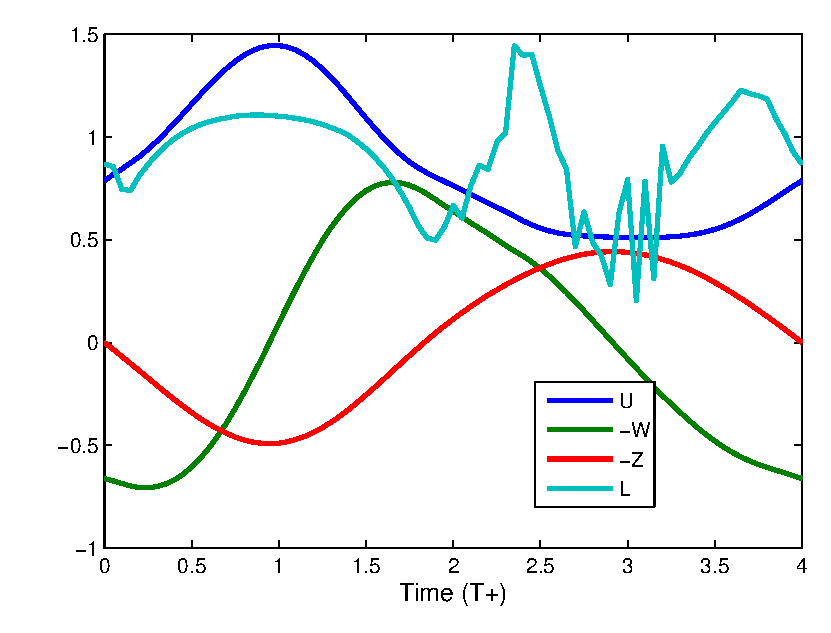
\includegraphics{./Figures/Windtype=1_Tg=4_Wg=0p129_quad_G=20.eps}}
  \end{center}
  \caption{Optimization results for a $4T$ long vertical gust}
  \label{fig:Validation_optimization}
\end{figure}

\FloatBarrier

Lissaman, with is optimal lift to drag ratio of 20 found a wind gust amplitude of $0.129$. 
Here the minimum required for neutral energy loop is $0.128$ (see figure \ref{fig:Validation_optimization}).
The shape of the state and control parameters curves are also consistent with the Lissaman results.

\par Similarly an optimization is performed for a purely horizontal wind gust.

\begin{figure}[h]
  \begin{center}
    \scalebox{0.8}
    {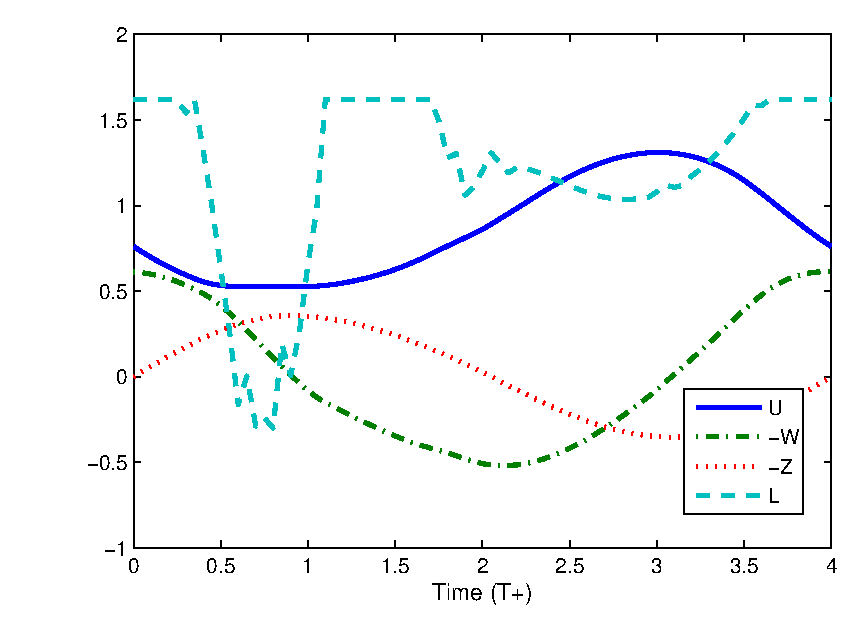
\includegraphics{./Figures/Windtype=2_Tg=4_Wg=0p246_quad_G=20.eps}}
  \end{center}
  \caption{$4T$ long horizontal gust for $G=20$, $W_a=0.246$}
  \label{fig:Horizontal_optimization}
\end{figure}

The resulting minimum wind amplitude is higher than for the vertical gust. 
However this shows that it is possible to take advantage of horizontal wind gusts to save energy if the performances are high enough.

\par Finally a combined horizontal and vertical gust is simulated.

\begin{figure}[h]
  \begin{center}
    \scalebox{0.8}
    {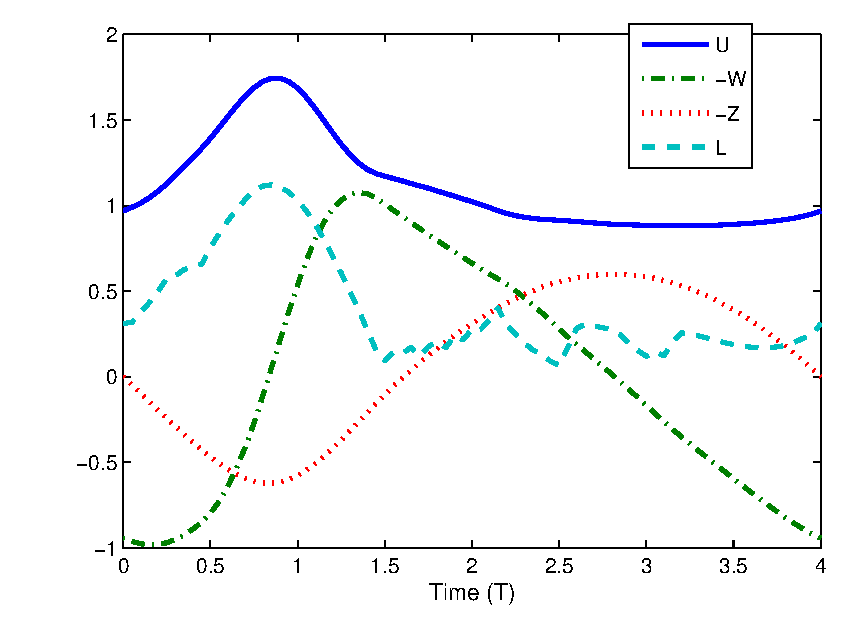
\includegraphics{./Figures/Windtype=3_Tg=4_Wg=0p232_quad_G=20.eps}}
  \end{center}
  \caption{$4T$ long combined gust for $G=20$, $W_a=0.232$}
  \label{fig:combined_optimization}
\end{figure}

Unsurprisingly the neutral energy loop trajectory exists also for this case.

\FloatBarrier

\Subsection{Typical results for the NACA0009 wing}

\par A similar batch of optimizations is done with the more realistic lift and drag profiles.
However since the lift to drag ration is lower than what Lissaman used in his model a higher gust amplitude is expected.

\begin{figure}
  \begin{center}
   \scalebox{0.8}
   {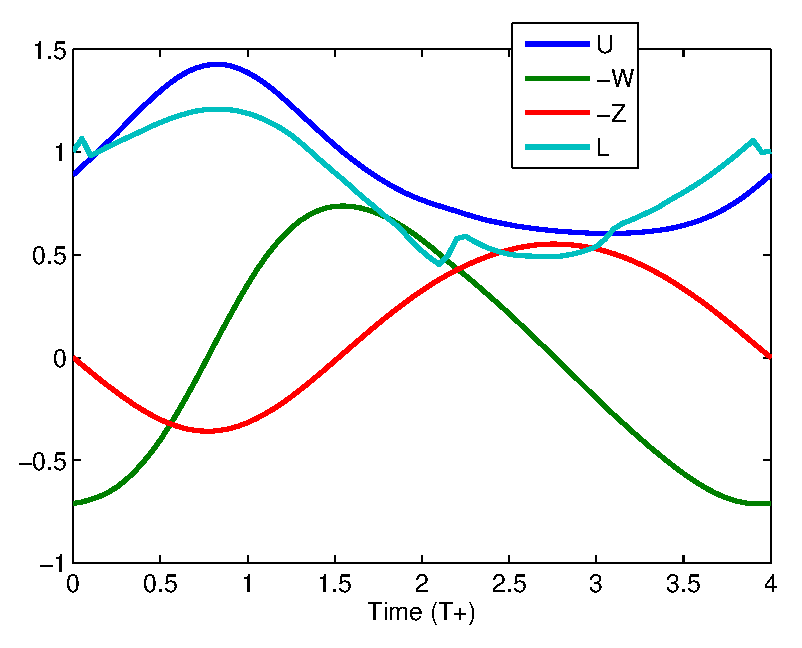
\includegraphics{./Figures/Windtype=1_Tg=4_Wg=0p205_UAV_alphamax=12.eps}}
  \end{center}
  \caption{$4T$ long vertical gust for UAV, $W_a=0.205$}
  \label{fig:vertical_optimization_UAV}
\end{figure}


\begin{figure}[h]
  \begin{center}
    \scalebox{0.8}
    {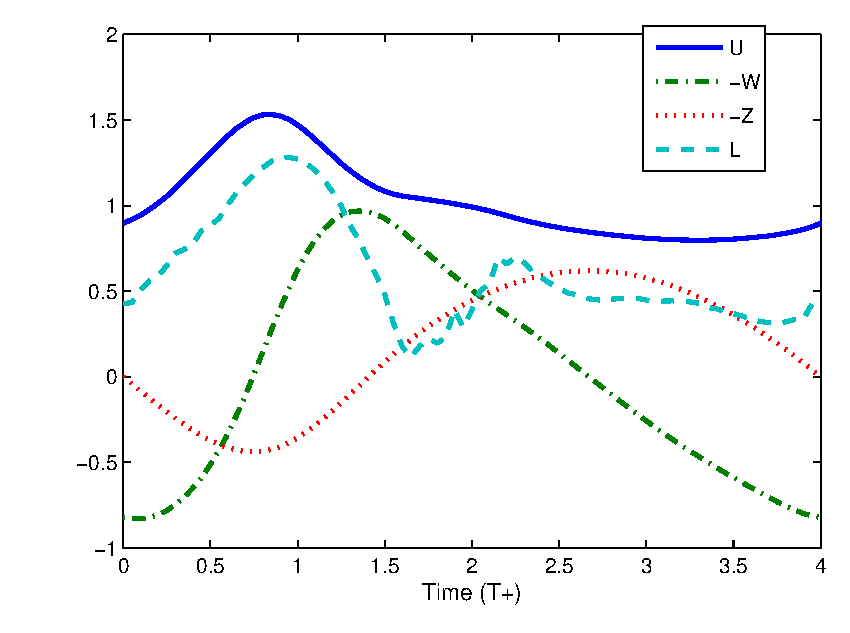
\includegraphics{./Figures/Windtype=3_Tg=4_Wg=0p387_UAV_alphamax=12.eps}}
  \end{center}
  \caption{$4T$ long combined gust for UAV, $W_a=0.387$}
  \label{fig:combined_optimization_UAV}
\end{figure}

As it can be seen on the figures \ref{fig:vertical_optimization_UAV} and \ref{fig:combined_optimization_UAV} the trajectories are similar in shape. However the gust amplitude needed to achieve neutral energy flight are a lot higher.
Such differences can be explained by looking at the maximum lift to drag ratio for both conceptual aircraft.
The quadratic drag profile used by Lissaman has a $G_{max}$ of 20.
The notional UAV used is closer to 14.

\FloatBarrier

\par With this kind of performances, a purely horizontal gust can't sustain a neutral energy loop.


\par To account for these differences a third batch of simulation is performed with by setting the $G_{max}$ parameter in the quadratic drag profile to 13.3.

\begin{figure}[ht]
  \begin{center}
    \scalebox{0.8}
    {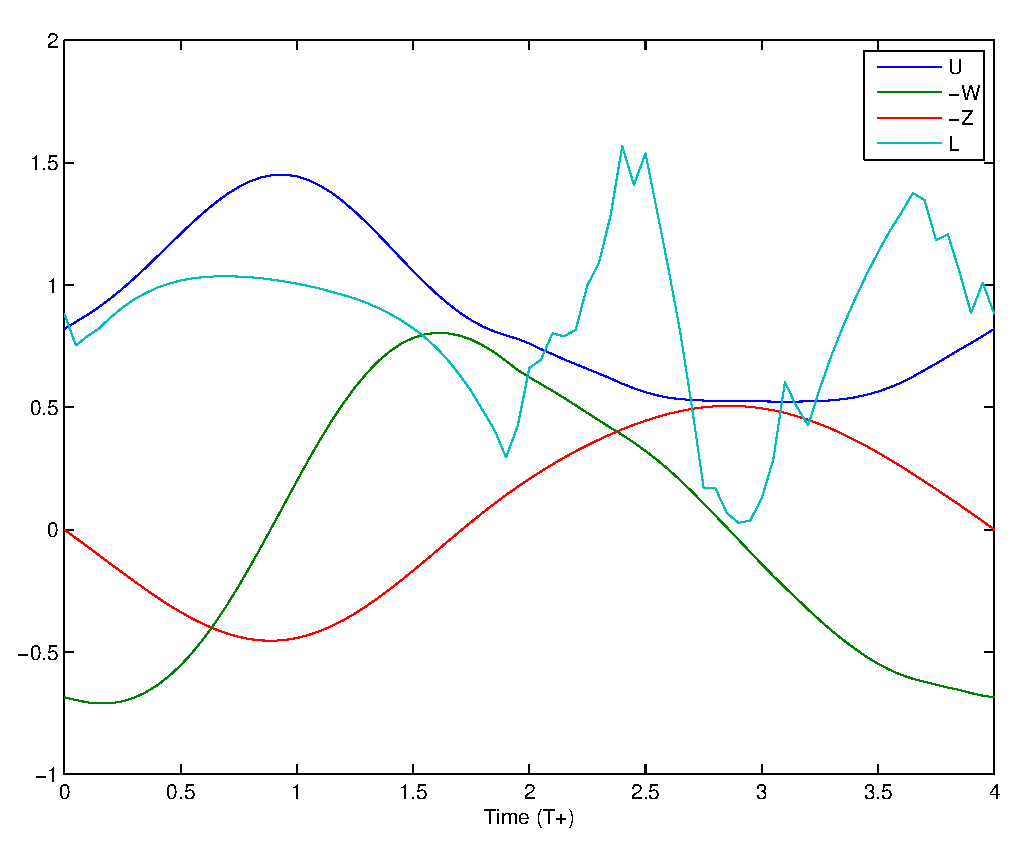
\includegraphics{./Figures/Windtype=1_Tg=4_Wg=0p194_quad_G=13.eps}}
  \end{center}
  \caption{$4T$ long vertical gust for $G=14$, $W_a=0.194$}
  \label{fig:vertical_optimization_UAV_modified}
\end{figure}


\begin{figure}[ht]
  \begin{center}
    \scalebox{0.8}
    {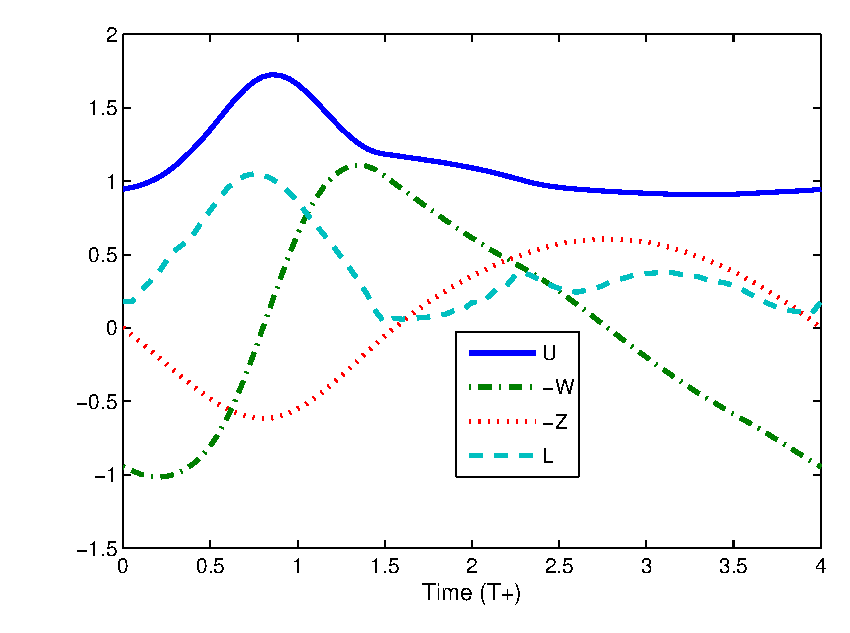
\includegraphics{./Figures/Windtype=3_Tg=4_Wg=0p360_quad_G=13.eps}}
  \end{center}
  \caption{$4T$ long combined gust for $G=14$, $W_a=0.360$}
  \label{fig:combined_optimization_UAV_modified}
\end{figure}

\par The results are similar.
Since the quadratic lift to drag profile isn't that different to the UAV one, the optimized gust amplitude is relatively close for both case.

\FloatBarrier

%\par Now that we have shown that for each type of trajectories the general behavior is the same, independently of the lift to drag ratio, it is interesting to compare at what time the energy was gained and at what rate it was changing.
%
%\par In the following figure the potential energy and kinetic energy are dissociated to highlight the actual effects of the altitude and speed gain.

% Do I want to make a trajectory/vector graph ??


\Subsection{Influence of the gust duration}
From our literature review it seems like most of the studies done on gusting winds has been conducted on gusts duration greater than $2T$.
Considering shorter gusts seems unreasonable of you only consider quasi steady aerodynamics, a $2T$ gust is about 2 seconds for vehicle flying 10 m/s.
However since the purpose this research is to extend the energy extraction envelope, such cases should be considered.

\begin{figure}[h!]
  \begin{center}
%    \scalebox{0.8}
%    {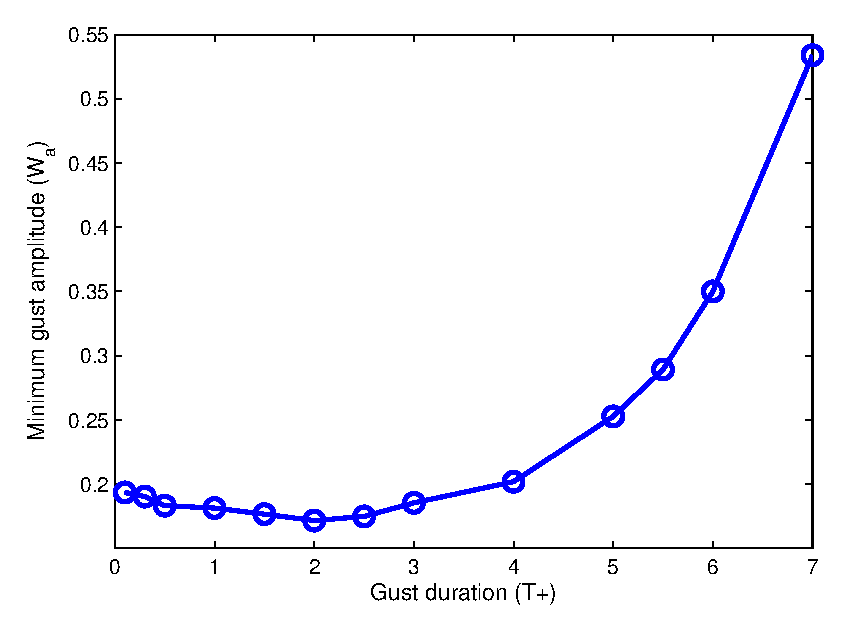
\includegraphics{./Figures/Vertical_gust_amplitude_vs_duration.eps}}
  \end{center}
  \caption{Influence of gust duration on the minimum gust amplitude for vertical gusts}
  \label{fig:vertical_amplitude_duration}
\end{figure}

\begin{figure}[h!]
  \begin{center}
%    \scalebox{0.8}
%    {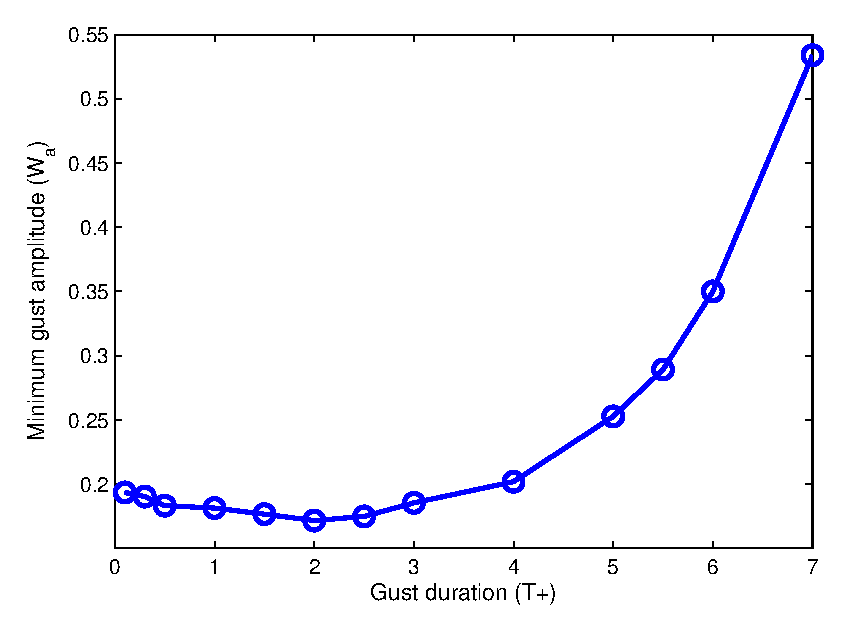
\includegraphics{./Figures/Vertical_gust_amplitude_vs_duration.eps}}
  \end{center}
  \caption{Influence of gust duration on the minimum gust amplitude for combined gusts}
  \label{fig:combined_amplitude_duration}
\end{figure}

\par Interestingly shorter gusts require less wind amplitude than the long ones.
This seems to indicate that most of the lost energy is due to the non-conservative drag force and not due to the downwind effects.
However the actual minimum gust amplitude required for neutral energy flight has a minimum for $2T$ long vertical gusts.

\par In figure \ref{fig:combined_amplitude_duration} This time no minimum is found.
This seems to reinforce the idea that the losses are mainly due to the energy dissipated by the drag since in this case the drag influence is mitigated by the horizontal component of the combined gust.

\par The diminishing gust amplitude required is an interesting phenomenon but can be fairly easily explained.
For a glider the only energy dissipation comes from the drag, in the cases we are considering the energy loss can be seen as a superposition of the losses due to simple cruse flight and the ones due to the maneuvering.
Since the total flight time during short gusts is shorter while the relative wind velocity remains more or less constant, the energy loss due purely to flying this long should be proportional to the flight time.
The energy input for this system is the wind gust itself is proportional to the force on the fluid times its velocity and the gust duration.
Since the force required to move the fluid is itself proportional to the derivative of the gust velocity the energy of the gust over a whole gust is in fact only proportional to the square of the gust amplitude.

\par This means that if the energy extraction efficiency was constant the value of $\frac{T_g0}{{W_g0}^2}$ should be constant for all the cases.


\begin{figure}[h!]
  \centering
  %\includegraphics{<+file+>}
  \caption{Energy extraction effectiveness}
  %\label{fig:<+label+>}
\end{figure}



\FloatBarrier


% get some commentary there

\Subsection{Influence of phase variation in the combined gust case}
For combined vertical and horizontal gusts another parameter can be changed.
So far the phase between the two components of the gust has been constant.

\par For this we define the phase $\phi$ as:

\begin{equation}
  \begin{array}[c]{c}
    W_g=W_a cos(2\pi T) \\
    U_g=W_a sin(2\pi T + \phi)
  \end{array}
  \label{eqn:combined_gust_phase}
\end{equation}

After Simulations are performed by 10 degrees steps with the following results.

\begin{figure}[ht]
  \begin{center}
    \scalebox{0.8}
    {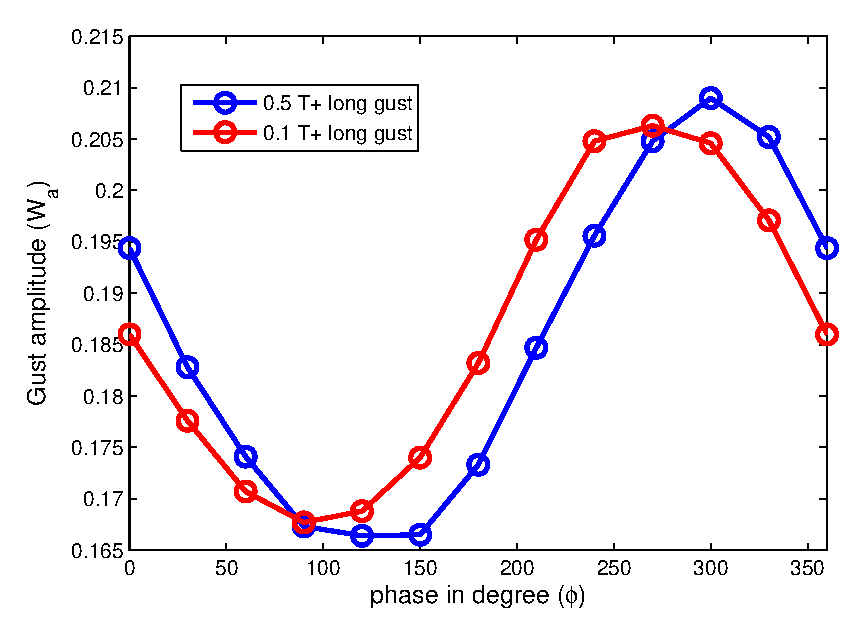
\includegraphics{./Figures/combined_gust_amplitude_vs_phase.eps}}
  \end{center}
  \caption{Influence of the phase between the component of the combined gust}
  \label{fig:combined_amplitude_phase}
\end{figure}

\par This clearly shows that our minimum gust amplitude for a 0 phase was actually close to the worst case possible.
The best case scenario is when the phase is around 90 to 120 degrees and the worst is around 270 to 300.

\FloatBarrier

\par We can see that the results are different for different gust durations.
One possible explanation for this is that at some point the inertia is too great and start to act as a low pass filter, introducing some phase shift in the trajectory. 



\Subsection{Maximum lift available effects}

\Subsection{Additional remarks}
As noticed by Lissaman the exact shape of the lift input isn't really important.
In his paper he approximated the input with a simple sinusoidal with amplitude and phase control, similar inputs in this simulation have produced minimum gust amplitude similar to the previous results.
This raises the hope that even very basic controllers should be able to improve UAV endurance.

% [DO I WANT TO  CHANGE THE PHASE TO ACTUALLY TEST IT !!!!]

\par While these results are supposed to be the optimal solution, it does not mean a controller can achieve such performances.
Even if the trajectory and lift curves are physically possible, the optimization algorithm assume a known gust shape and optimize all of the time points at once.
This means that contrary to a real controller the optimized trajectory can anticipate the wind change and preventively react.
Even if the wind gusts were perfectly sinusoidal, since a controller is casual it would not be able to anticipate.
Finally in a real life scenario the wind would of course not be a simple sinusoidal gust.

\par The simulation is also limited by its inability to account for the moment of inertia along the pitch axis.
Even is part of the lift change can be handled by the active flow control system, at low angle of attack, most of the lift comes from the changes in $\alpha$.

\par Even with all this limitations these results provide good insight into what would be needed implement energy extraction trajectories in UAVs.



\Subsection{Horizontal gusts}

\Subsection{Vertical gusts}

\Subsection{Combined gusts}



\Subsection{Preliminary analysis of the results}

\Chapter{Active Flow Control}

\Section{Experimental setup}

\Subsection{wind tunnel}

\Subsection{Leading edge piezoelectric actuators}

\par{NACA 009 airfoil with leading edge synthetic jets}

\par{Driver for the piezoelectric elements}

\Section{Single pulse response}

\Subsection{Pulse design}
% high frequency to frive the piezos (find paper for that)

\Subsection{Influence of the pulse duration}

\Subsection{Effect of pulse duration}

\Subsection{Effect of pulse separation}

\Subsection{Effect of pulse amplitude}


\Section{Pulse train design}

\Subsection{Design constraints}
% bandwidth consideration

\Subsection{Chosen parameter}

\Subsection{Square input example}




\Section{Experimental results for different input signals}

\Subsection{continual and square input signals}

\Subsection{triangle input signal}

\Section{System identification}
% discuss about dead time, lift reversal, asymmetry

\Chapter{Modelization of the Lift coefficient under unsteady pitching motion}

%servo drive and stuff

\Section{Theoretical background of the GK model}

\Section{GK model adaptation}

\Subsection{Steady list and stalling behavior}

\Subsection{State variable approximation}

\Section{Experimental Setup}

\Section{Model validation}
% put both sinusoidal and ``random'' motion

\Chapter{Controller design and validation}

\Section{Proof of concept for combining AFC with pitching}

\Subsection{Open loop experimental results}

\Subsection{Comparison with models output}

\Section{Controller structure}

\Subsection{AFC transfer function inverse}

\Subsection{Controller input and objective discussion}

\Subsection{Controller block choice}

\Section{Results}

\Subsection{Periodic pitching motion}

\Subsection{Limited bandwidth random pitching motion}

\Section{Discussion of the results}

\Subsection{Bandwidth limitation}

\Subsection{Precision issues}

\Section{Possible improvements and feedback implementation}

\Chapter{CONCLUSION}

% \Section{Low order model for unsteady flow}

\par The Goman and Khrabrov model shows good agreement in both shape and magnitude for the lift and drag of a pitching airfoil in a wide range of conditions.
It is fast and light and can be adjusted to a new airfoil (or even a whole aircraft) without requiring extensive experimental studies.
In fact in theory only a static map and one unsteady case should be enough to obtain the whole model.

\par The work in this thesis has proven that the drag can also be easily modeled and there is little doubt that the moment coefficient $C_m$ could be modeled too.

\par Implementing this model is simple enough that it can be used in computationally heavy applications such as optimization problems or real time applications.
It is however non-linear and as such isn't easily invertible or analyzable with traditional control system methods.

\Section{Energy extraction optimization}

\par From the results presented in this thesis it can be seen that energy extraction can be performed for complex temporal wind gusts with vertical and horizontal components.
In these gusts overall neutral energy trajectories are possible and require less and less wind gust amplitude the shorter the gust is.
For short gust ($T_g \le 3$) high angles of attack are needed for maximum performance, which can lead to flow separation.

\par The introduction of an unsteady aerodynamic model is possible and proves necessary when gusts are very short ($T_g \le 0.7$ or $k \ge 0.05)$).
At this point unsteady effects such as lag in the flow separation can be observed and even taken advantage of.
While the maneuvers required to obtain such trajectories are unlikely to be realistically done on aircrafts, these results could be exploited in vertical wind turbine pitch optimization for example.
The results for gusts shorter than $T_g=0.2$ ($k=0.175$) are less obvious to interpret and will require further study, perhaps with a problem more representative of the system operating at such frequencies.

\par While these results shows the optimal trajectory found by the algorithm it is important to keep in mind that the algorithm optimize the trajectory globally over the whole period.
This means that it can take preemptive actions because it ``knows'' what will happen later in time.
A real controller flying in an environment where the wind gust shape can't be predicted would not be able to reach the same energy extraction performances.

\Section{Possible improvements and additional work}

\par One of the weakness of the optimization with the GK model is that it does not account for the unsteady effects due to the surging and gusting components of the relative wind.
I believe that the GK model could be modified to include these effects but a complete experimental campaign would be needed.

\par The ``staircase'' effect described in section \ref{sub:staircase} could be mitigated by introducing a more realistic model for the aircraft dynamics that include the moment of inertia.
Going even further, a basic elevator model could be implemented.

\par Finally replacing the temporal wind profile by a spatial one would allow for the use of more realistic and complex wind fields.



\Section{Summary}

This was just to create a sample section...

\clearpage


%
% APPENDIX
%

% Do the settings of appendices with \appendix command
\appendix

% Then create each appendix using
% \Appendix{title_of_appendix} command

\Appendix{Table of Transition Coefficients for the Design of
Linear-Phase FIR Filters}
Your Appendix will go here !

 \moretox

  \Appendix{Name of your Second
Appendix}

Your second appendix text....

\Appendix{Name of your Third Appendix}
 
Your third appendix text....
%
% BIBLIOGRAPHY
%
% you have two options: 1) create bibliography manually,
% 2) create bibliography automatically. See BibliographyHelp.pdf file for details.


\bibliographystyle{plain}
\bibliography{mybib}


\end{document}  % end of document
